\chapter{相关理论概述}
1970 年 Fukushima 等人\cite{fukushima1970electronic}在对生物视网膜结构的研究工作中,展示了首个电子视网膜离散模型,这种新颖的
获取信息的方式很快引起了相关领域学者们的兴趣,但是由于陌生的异步逻辑领域以及像素响应特征的不均匀性,
事件相机的发展一直处处受限,一直到2008年首部事件相机(DVS)问世,也是世界上第一台商用事件相机。此后,在经
过了十数年的发展,事件相机已经开发出了多种版本款式,应用针对不同的工作任务与场景,如ATIS,DAVIS,CeleX,
本次研究引入工作的是型号为DAVIS346的事件相机,后续都会在这款相机的基础上进行工作的开展,后续不再进行累述。

\section{事件相机}
\subsection{工作原理}
本文在前面也粗略地提起到了事件相机与传统可见光相机在原理与机制上的巨大不同。传统的可见光传感设备
为一次成像,图象是以一个固定的帧率被设备输出,每次成像过程中,相机的各个相素会进行电荷收集并在曝光
流程结束后将像素上的电荷信息转化为数字信号输出至外界。这种工作原理下,拍摄高速运动物体时缺陷就
极为明显,图像很容易就会出现模糊与失真,如图\ref{3}所示。事件相机就是这样一部为了解决该问题的,仿生物视网膜结构模型的
传感设备\cite{tayarani2021event},它由生物视网膜细胞具有对亮度瞬变的高敏感性获得启发,每一个像素独立地、仅会在对数亮度值的变化超出阈值时
进行一次输出。这种机制,给予了这类传感器更广的动态范围,也自动消除了环境中非变化物体等产生的冗杂信息。
\begin{figure}
    \centering
    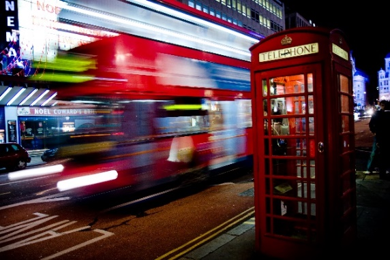
\includegraphics[width=\textwidth]{figures/motion_blur.png}
    \caption{失真}
    \label{3}
\end{figure}
\begin{figure}
    \centering
    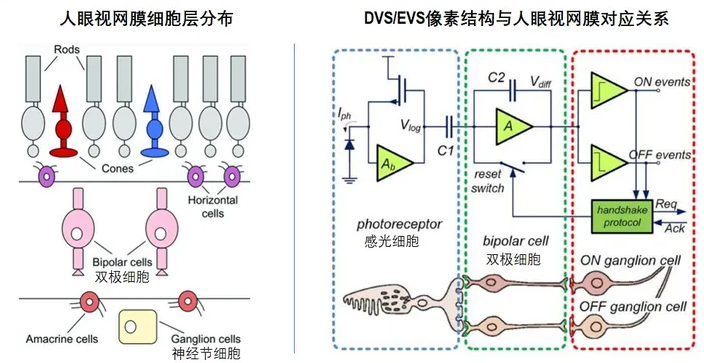
\includegraphics[width=\textwidth]{figures/working_principle.png}
    \caption{事件相机主要工作原理示意图}
    \label{2}
\end{figure}

事件相机内部工作模块主要由差分电路、感光器和比较仪三部分组成,实现对生物视网膜结构的
模拟,主要原理示意如图\ref{2}所示。对于生物而言,感受到光线后,它视网膜上的受体细胞受到相应的刺激,就会自发将光信息转变成神经信息,后段细胞还会分别筛选出亮部和暗部,经过
神经节细胞的处理后,信息就传递到了大脑皮层,呈现为视觉。而在事件相机中,光信息在感光器电路中会转换成电信号,它会通过放大器,最终由比较器根据
亮度变化进行分离,将光信息转化为“事件”信息,最后在经过一系列的后续处理后,转为图像输出。\cite{eibensteiner2017event}

假定亮度为I,事件相机中的亮度定义都是其对数值,即L=log(I),那么在某一个时刻$t_k$,某一个像素点$X_k=(x_k,y_k)$处的亮度改变就可以记为
\begin{equation} 
    \Delta L(X_k,t_k)=L(X_k,t_k)-L(X_k,t_k-\Delta t_k)
\end{equation}

其中,$\Delta t_k$是一个极小的时间间隔,如果亮度的变化$\Delta L$超出了相机所设定的阈值C,事件就会触发,这个过程也可以表示为
\begin{equation} 
    |\Delta L|>|p_kC|
\end{equation}

其中,$p_k=\pm1$表示极性,也就是亮度发生了正向(ON)或者负向(OFF)变化,本文所提及的事件数据就以$e_k(x_k,y_k,t_k,p_k)$这样一个形式输出出来,
可以看到,本文后续工作中所提起的“事件”,往往就是这样的一个四维向量(空间坐标、
时间坐标、极性),如图\ref{4}所示即为其空间表现形式。
\begin{figure}
    \centering
    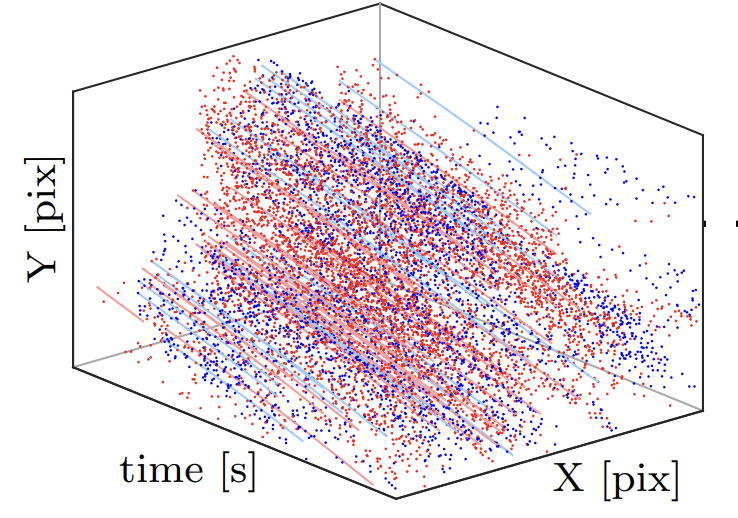
\includegraphics[width=0.6\textwidth]{figures/event_stream.png}
    \caption{二维平面事件点云}
    \label{4}
\end{figure}

\subsection{对事件数据的处理}
由于数据的异步性,基于事件的计算机视觉中的处理步骤与传统相机有很大不同。
事件表示是基于事件的计算机视觉架构的第一步,将原始 DVS 数据转换为时空格式,可由后续处理步骤(如深度
神经网络)执行分类、运动跟踪、预测、图像重建和六维自由度估算等任务。

目前可以将事件表征大致分为四种种模式。第一种模式是脉冲处理,如 SNN,
它天生支持稀疏的异步数据,但脉冲形式的机器学习在功耗和方法上都不太理想,学习的灵活性和训练成熟度都不如传统的 CNN,比传统的 CNN 更难训练。
它们还需要专门的硬件,而大多数计算平台都不具备这些条件。第二种
是分析事件处理,即明确利用事件的时序和极性,例如局部平面拟合和时间导数插值。
然而,大多数分析事件表示法都是针对特定任务的,因此不容易推广到广泛的应用中。
第三种模式是以同步形式与机器学习方法配对,利用 CNN 的飞速发展,将事件数据转换为类似二维图像或三维视频帧的代理,
本文称之为 "事件帧"。虽然仅使用几个事件帧不可能无损地表示异步事件数据,但本次工作的注意力集中在事件在每个像素点的时空演变。
第四种模式是亮度图像重建,通过使用事件估算每个像素的亮度值,在传统图像上训练的机器学习方法
可以直接利用。\cite{baldwin2022time}

在事件的同步表示法中,大多数方法都采用了时间窗口来对接收到的事件进行分组。
窗口可以是一个固定的时间间隔,以产生恒定的帧速率事件帧,也可以是一个固定的事件编号,以产生自适应帧速率。
在一种称为 "事件累积 "或 "事件计数 "的表示方法中,时间窗口内的事件按极性分开,并对每种极性类型的事件进行计数,从而得到
两个大小为 H ×W 的图像。虽然这种方法保留了极性信息,但会丢失时间信息。类似的方法还有 "极性求和",通过对给定时间窗口内的事件极性求和来计算,通过观察发现
正或负事件的数量越多,强度变化(即边缘)就越大。极性求和产生一个单一的 H × W 事件帧,
近似于给定时间窗口内发生的整体强度变化。

使用时间窗口的方式也有多种,一种称为 "体素化网格 "的表示方法采用了一种时间量化方法,使用双线性采样核
将事件映射到最近的时间网格上;不过,当多个事件被映射到同一量化像素时,信息就会丢失。
事件脉冲张量(EST)是体素化网格的一种变量,在极性上进行了分离,并允许在每个体素上执行任何
功能,而不仅仅是极性信息的总和。时间量化方法的一个缺点是,它对时间并非不变,这意味着初始化时间的变化
会对同一数据集产生不同的表示。

时间表面是事件累积和极性求和表示法的替代方法\cite{benosman2013event},它优先考虑事件发生的时间,而不是
边缘幅度。时间表面是一种二维表示法,将时间戳编码为像素值。活动事件表面
(SAE)的时间表面保留了每个像素位置(每个极性)上最新事件的时间。
这对于慢动作序列或低光照环境下的成像并不理想,因为事件发生的时间变得模糊不清,或被噪音干扰。所以可以
利用单个边缘产生多个事件这一事实来提高稳定性。感知时间表面是一种
是一种混合方法,借鉴了时间表面和极性求和法。感知时间面滤波的目的是去除不成组出现的事件(因为单个边缘的事件是不成组出现的),
并报告第一个事件时序(对应边缘到达时序)和在这些组中发生的事件数(与边缘幅度相对应)。
这样可以过滤孤立的事件(即噪声),保留了更高保真度的时间信息以及边缘幅度,但舍弃了将被过滤掉的低对比度变化,
在实时应用中会带来延迟。

其他方法使用基于紧凑图的表示法,基于图的方法将时间窗口内的事件转换为一组连接的节点,U × V。
这种紧凑的表示方法可以减少计算和内存资源,保持事件摄像机的数据稀疏性。不过,构建图谱需要大量计算资源。此外,这种表示法在处理过程中会丢弃精细的
时空信息。

时间窗口或事件窗口表示法的一个普遍问题是,它们会导致延迟。对于具有固定帧频的时间窗口
表示时,在窗口早期发生的事件在时间窗口结束前不会被评估。事件
窗口表示法的计算效率更高,但由于事件窗口表示法没有延迟上限,完全基于传感器的事件速率,
通常需要预定义的窗口大小,如果没有网络再训练,就无法更改窗口大小。



\subsection{事件相机的独特优势}
基于上述篇幅介绍的事件相机的独特机制,事件相机相对于传统可见光传感器有着下列的先天优势:

1.高时间分辨率。由于各相素独立工作的机制,省去了传统可见光相机的很多中间流程,可以达到微秒级分辨率,几乎不会出现
运动模糊。

2.低数据量。每个像素当且仅当变化超出阈值才会输出一次,很多无用的干扰信息都会被机制自动剔除,因此事件相机的输出数据远远
低于传统设备,在处理速度等很多方面就有着很大优势。

3.低功耗。由于2的原因以及事件相机不需要模数转换器读取像素,后续的处理功耗也自然较低,往往是毫瓦级,与传统设备有百倍以上的差距。

4.高动态范围。由于采用对数制光强,事件相机往往可以达到传统相机2倍以上动态范围,可以适应很多欠曝和过曝场景。

\section{机器学习}
机器学习是一种人工智能的分支,它致力于研究如何让计算机系统通过从数据中学习经验,从而改善执行特定任务的性能,而无需明确地编程。
机器学习的目标是设计和开发能够自动学习的算法和模型,使计算机可以从数据中发现模式、生成规则、做出预测,并最终执行任务。

机器学习的基本理念是从数据中学习。它依赖于大量的数据作为输入,通过数据来发现问题的解决方案,而不是人为地指定规则。
在机器学习中,数据被抽象为不同类型的模型,这些模型可以是线性模型、非线性模型、神经网络等。模型通过调整其参数以最好地拟合数据,从而学习数据中的模式和规律。
机器学习算法通过学习过程来调整模型的参数,使其能够捕捉数据中的特征和模式。学习过程通常分为训练阶段和推理/预测阶段,训练阶段使用已知的数据来调整模型,推理/预测
阶段则用于对新数据进行预测或分类。机器学习模型的泛化能力是评估其性能的关键指标。泛化能力指的是模型对未见过的数据的适应能力。一个好的机器学习模型应该能够在训练数据之外的数据上表现良好。

对于火焰检测工作,更多的是一种火焰有无的二分类问题,对于此类问题,在机器学习领域常常利用支持向量机来处理。支持向量机(Support Vector Machine, SVM)是一种用于分类和回归分析的监督学习模型,
它在机器学习领域有着广泛的应用。SVM 的基本原理是构建一个将输入空间划分为不同类别的超平面,使得不同类别的数据点在空间中有尽可能大的间隔。
\subsection{SVM的发展}
SVM最早于1982年由Vladimir Vapnik和Alexey Chervonenkis提出\cite{stitson1996theory},并在1982年至1992年之间发表了一系列论文,其中最具代表性的是在1992年发表在IEEE TPAMI杂志上的论文《统计学习理论》。
1992年,Vapnik和其同事首次提出了线性SVM的概念,并将其应用于二分类问题\cite{chapelle1999support}。线性SVM的基本思想是在特征空间中找到一个最优的超平面,将不同类别的样本分开,使得间隔最大化。同时,在上个世纪90年代中后期,
SVM在模式识别、文本分类等领域开始受到广泛关注。随后,Vapnik和其同事将SVM扩展到了非线性分类问题,引入了核函数的概念,\cite{cortes1995support}通过将数据映射到高维空间使其线性可分。
1992年,Corinna Cortes和Vladimir Vapnik提出了使用径向基函数(Radial Basis Function, RBF)作为核函数的SVM,极大地拓展了SVM的应用范围。
21世纪初,随着机器学习和数据挖掘技术的发展,SVM作为一种强大的分类和回归工具开始在实践中得到广泛应用。它在图像识别、文本分类、生物信息学、金融预测等领域展现出了卓越的性能,
已经成为了机器学习领域中最为重要的算法之一,其理论基础和实际应用在学术界和工业界都受到了广泛的认可和应用。
\subsection{SVM相关概念介绍}
SVM 的核心思想是在高维空间中找到一个最优的超平面,将不同类别的数据点分隔开来。该超平面使得距离超平面最近的数据点到超平面的距离(即间隔)最大化。
SVM 能够处理线性可分和线性不可分的数据集。对于线性不可分的情况,通过引入核函数将数据映射到高维空间中,从而使其在高维空间中线性可分。
在回归问题中,SVM 则是利用支持向量回归(Support Vector Regression, SVR)进行预测,通过找到一个超平面,使得数据点与超平面的距离尽可能小,并且满足一定的容差范围。
核函数是 SVM 的重要组成部分,它用于将数据从原始特征空间映射到更高维的特征空间,以便在新的特征空间中实现线性可分。常用的核函数包括线性核函数、多项式核函数、高斯核函数(径向基函数)等。
SVM 中的参数包括惩罚参数 C、核函数的参数、容差范围等。这些参数的调节对于模型的性能和泛化能力有着重要影响。通常可以通过交叉验证等方法来选择最优的参数。






\section{本章小结}
本章详细介绍了事件相机的工作原理,介绍了它的独特机制和数据形式,介绍了应用工作中对事件数据的一些常见处理方法,
并且介绍了其相对于传统相机的几个显著优点。同时本章也对后面涉及到的机器学习和支持向量机的一些相关概念进行了讲解,
对相关的工作结构原理进行了阐述。后面的章节,我们将利用事件相机开展并介绍本次的主要工作进程。